\documentclass[./]{subfiles}

%NURBS
\begin{document}
Finally, the functions we will use to describe our surface along with being the basis for analysis are the Non-Uniform Rational B-Splines (NURBS). In one dimension, NURBS are defined as ratios of of B-spline bases:
\begin{equation}
R_i(\xi) = \frac{w_i N_{i,p}(\xi)}{\sum_{b=1}^{n} w_b N_{b,p}(\xi)}, i = 1, \dots, n.
\end{equation}
NURBS can be built up into higher dimensions in exactly the same tensor product fashion as B-spline bases. 

NURBS are used extensively in computer graphics, as they provide a means of exactly producing conic sections such as circles and ellipses \cite{piegl_nurbs_2012}. In Figure \ref{fig:cylinder}, we use the 3D modeling program Blender to generate a cylinder. The set of vertices surrounding the cylinder are the control points making up the \textit{control mesh} of the surface. 
\begin{figure}[!htbp]
  \centerline{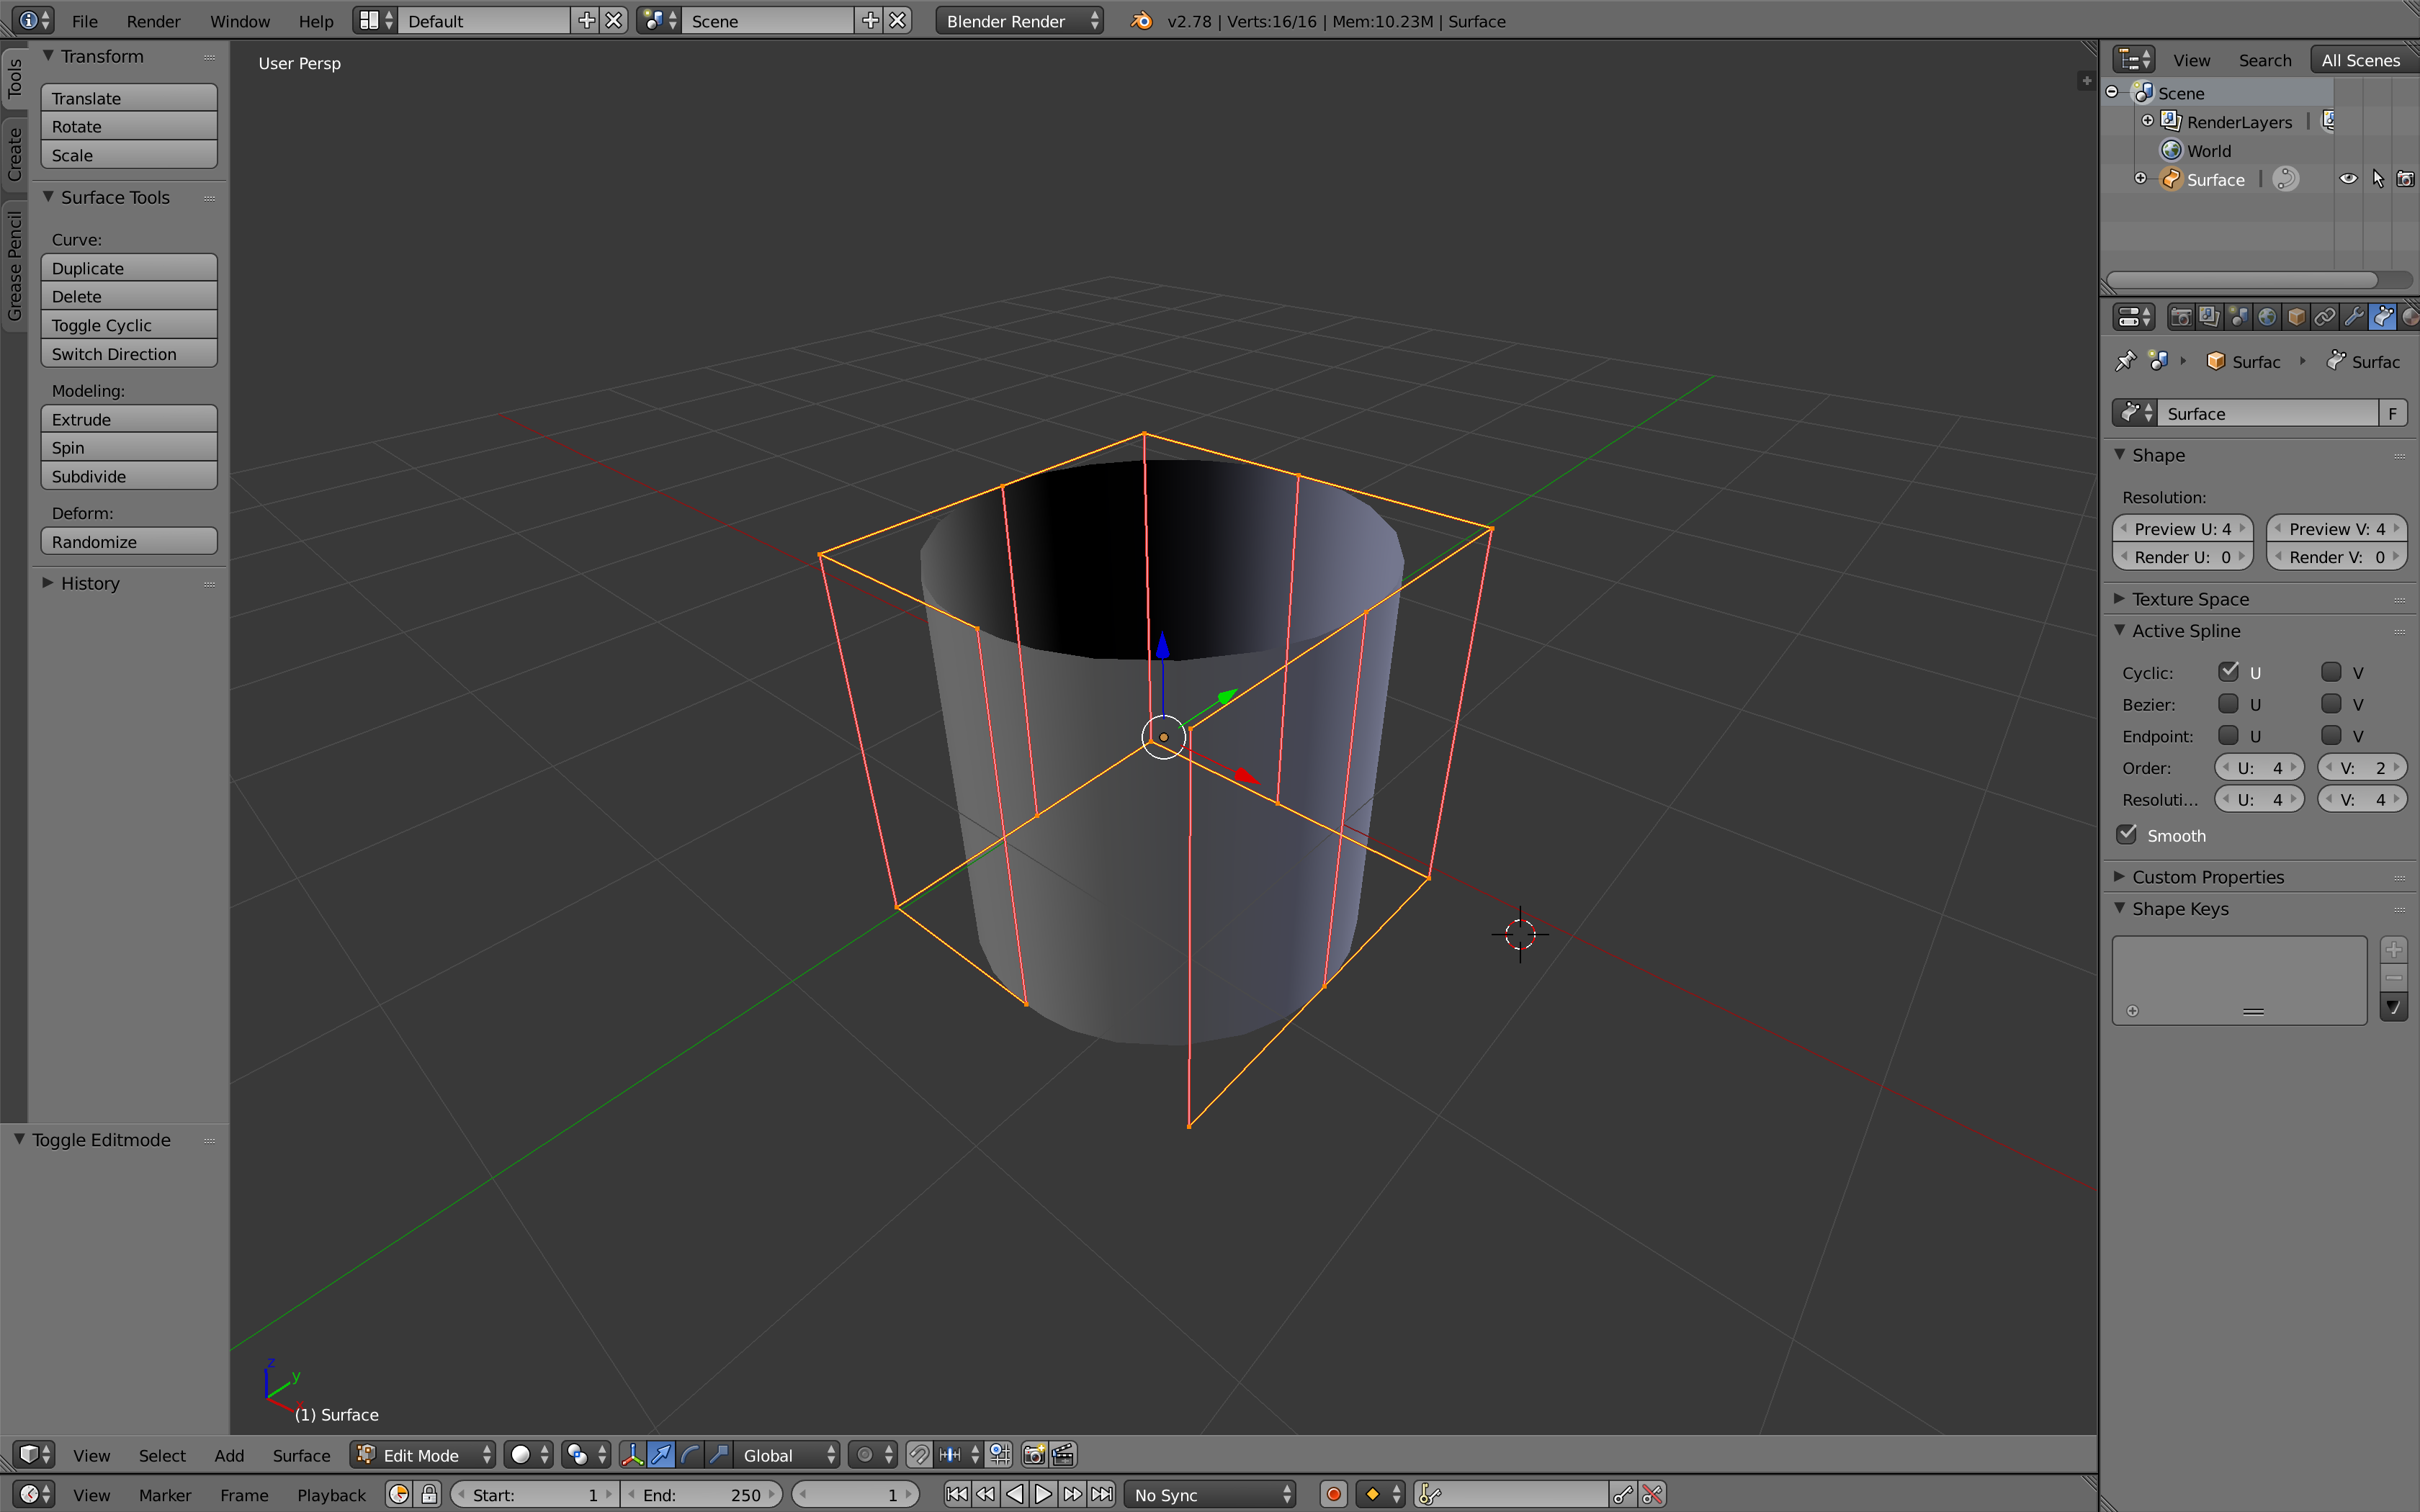
\includegraphics[width=4in]{./figures/CylinderBlender}}
  \caption{NURBS cylinder created in Blender}
  \label{fig:cylinder}
\end{figure}

\end{document}